\documentclass[conference,a4paper]{IEEEtran}
\IEEEoverridecommandlockouts

\usepackage{cite}
\usepackage{amsmath,amssymb}
\usepackage{graphicx}
\usepackage{array}
\usepackage{booktabs}
\usepackage{url}
\usepackage{tikz}
\usetikzlibrary{positioning,fit,arrows.meta,calc}

\begin{document}

\title{Designing an AI Gateway for the Serbian AI Factory Antenna: Functional Scope and Candidate Technologies%
\thanks{This work has received funding from the European High Performance Computing Joint Undertaking (JU) under Grant Agreement No.~101263280 (SAIFA).}}

\author{
\IEEEauthorblockN{Aleksandra Stojanovi\'c}
\IEEEauthorblockA{\textit{School of Electrical Engineering} \\
\textit{University of Belgrade}\\
Belgrade, Serbia \\
sa230234d@student.etf.bg.ac.rs}
\and
\IEEEauthorblockN{Dimitrije Pe\v{s}i\'c}
\IEEEauthorblockA{\textit{School of Electrical Engineering} \\
\textit{University of Belgrade}\\
Belgrade, Serbia \\
pd230014d@student.etf.bg.ac.rs}
\and
\IEEEauthorblockN{Zaharije Radivojevi\'c}
\IEEEauthorblockA{\textit{School of Electrical Engineering} \\
\textit{University of Belgrade}\\
Belgrade, Serbia \\
zaki@etf.rs}
}

\maketitle

\begin{abstract}
The EuroHPC AI Factories initiative is building a European network of AI-optimised supercomputing centres, complemented by AI Factory Antennas that extend their services to countries without large-scale AI infrastructure. This paper presents the design of the AI Gateway of the Serbian AI Factory Antenna (SAIFA), the single entry point through which researchers, industry, public institutions and learners reach national computing resources, datasets, models, workflows, training and support, and through which these resources are linked with the Pharos and IT4LIA AI Factories. The Gateway is conceived as a modular integration and control layer rather than a monolithic platform. We define its functional scope, elaborate the main functional areas, and map each area to candidate open-source components, identifying the integration logic that has to be developed specifically for SAIFA. A two-step technology-selection method and a proof-of-concept baseline for the beta release are also outlined.
\end{abstract}

\begin{IEEEkeywords}
AI Factory, AI gateway, EuroHPC, high-performance computing, MLOps, federation, science gateway.
\end{IEEEkeywords}

\section{Introduction}

Access to large-scale computing has become a precondition for modern artificial intelligence (AI) research and innovation. To make such access available across Europe, the EuroHPC Joint Undertaking launched the AI Factories initiative, in which hosting sites operate AI-optimised supercomputers together with services for data, models, training and user support~\cite{eurohpc_aif}. In October 2025, 13 AI Factory Antennas were selected to extend these services to further countries; each Antenna is linked to one or more AI Factories~\cite{eurohpc_antennas}.

The Serbian AI Factory Antenna (SAIFA) is one of them~\cite{cordis_saifa}. It runs from May 2026 to April 2029, builds on national infrastructure---the PARADOX HPC cluster at the Institute of Physics Belgrade and the AI computing infrastructure of the Institute for AI Research and Development of Serbia (ITE)---and is linked with the Pharos (Greece) and IT4LIA (Italy) AI Factories. Its target application domains are language and culture, energy and manufacturing, health, and environment.

The user-facing element of SAIFA is the \emph{AI Gateway}. Similar to science gateways that expose grid and HPC resources through community-specific interfaces~\cite{wilkinsdiehr2007}, the Gateway must hide infrastructural complexity, but it must also cover the full AI lifecycle and interoperate with partner AI Factories. This paper summarises the initial Gateway design~\cite{saifa_d31}. Its contributions are: (i)~a positioning of the Gateway within the AI Factory ecosystem, (ii)~a structured functional scope derived from domain user stories and system use cases, (iii)~an elaboration of the main functional areas, and (iv)~a mapping of these areas to candidate tools together with a selection method.

\section{AI Factories, Antennas and the Role of the Gateway}

AI Factories are built around EuroHPC supercomputers and provide compute capacity, AI-ready data, model development environments, training and expert support~\cite{eurohpc_aif}. Antennas do not replicate this infrastructure. They provide national access points, local expertise and smaller-scale computing, and channel demanding workloads and validated assets to the linked AI Factories. In addition, European assets are discoverable through the AI-on-Demand Platform~\cite{aiod}.

SAIFA follows this model through four layers (Fig.~\ref{fig:structure}). The \emph{infrastructure} layer comprises PARADOX and ITE compute and storage, connected by a planned 100\,Gb/s link established with AMRES. The \emph{computing environment} layer provides containerised AI frameworks and notebooks. The \emph{AI Gateway} layer exposes models, datasets, tools, workflows, applications, training and support. The \emph{use case} layer contains the domain applications developed in the project. Development and preliminary testing are carried out on national infrastructure, while final validation and benchmarking use the Greek and Italian AI Factories.

\begin{figure}[t]
\centering
\includegraphics[width=\columnwidth]{fig_saifa_structure.jpg}
\caption{Layered structure of the Serbian AI Factory Antenna.}
\label{fig:structure}
\end{figure}

Within this structure the Gateway acts as \emph{middleware}: it accepts user or application requests, applies common identity, policy and metadata rules, and forwards each request to the appropriate connected service (Fig.~\ref{fig:arch}). The Gateway itself is responsible for identity and access enforcement, catalogue and metadata management, request validation and routing, quota checks, status aggregation, monitoring, audit and provenance. It does not replace schedulers, clusters, object stores, model-serving engines or learning-management systems. Domain logic, data preparation and interpretation of results remain the responsibility of domain applications or authorised user code.

\begin{figure}[t]
\centering
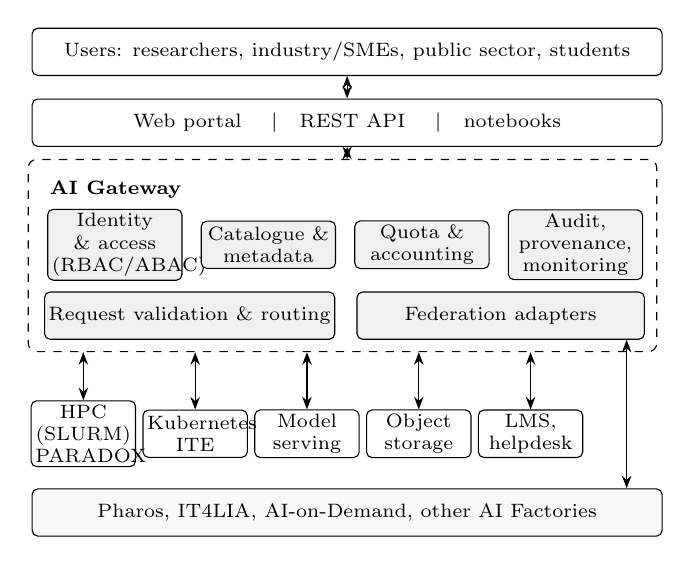
\begin{tikzpicture}[
  font=\scriptsize,
  box/.style={draw, rounded corners=2pt, align=center, minimum height=6mm, inner sep=1.5pt},
  core/.style={box, fill=gray!12},
  >={Stealth[length=1.6mm]}
]
% user-facing rows (total width 8.0 cm)
\node[box, minimum width=8cm] (users) at (4,0) {Users: researchers, industry/SMEs, public sector, students};
\node[box, minimum width=8cm] (portal) at (4,-0.9) {Web portal \quad\textbar\quad REST API \quad\textbar\quad notebooks};
% gateway core
\node[font=\scriptsize\bfseries, anchor=west] (gwt) at (0.1,-1.75) {AI Gateway};
\node[core, text width=1.6cm] (iam)   at (1.05,-2.45) {Identity \& access\\(RBAC/ABAC)};
\node[core, text width=1.6cm] (cat)   at (3.0,-2.45) {Catalogue \&\\metadata};
\node[core, text width=1.6cm] (quota) at (4.95,-2.45) {Quota \&\\accounting};
\node[core, text width=1.6cm] (audit) at (6.9,-2.45) {Audit, provenance,\\monitoring};
\node[core, minimum width=3.65cm] (route) at (2.0,-3.35) {Request validation \& routing};
\node[core, minimum width=3.65cm] (fed)   at (5.95,-3.35) {Federation adapters};
\node[draw, dashed, rounded corners=3pt, fit=(gwt)(iam)(audit)(route)(fed), inner sep=1.5mm] (gw) {};
% back-ends (x from 0 to 7.0 cm)
\foreach \n/\x/\t in {hpc/0.65/{HPC (SLURM)\\PARADOX}, k8s/2.07/{Kubernetes\\ITE}, serve/3.49/{Model\\serving}, store/4.91/{Object\\storage}, lms/6.33/{LMS,\\helpdesk}}
  \node[box, minimum width=1.3cm, text width=1.22cm] (\n) at (\x,-4.85) {\t};
\node[box, minimum width=8cm, fill=gray!5] (aif) at (4,-5.85) {Pharos, IT4LIA, AI-on-Demand, other AI Factories};
% links
\draw[<->] (users) -- (portal);
\draw[<->] (portal) -- (portal |- gw.north);
\foreach \n in {hpc,k8s,serve,store,lms} \draw[<->] (gw.south -| \n) -- (\n);
\draw[<->] (7.55,-3.35 |- fed.south) -- (7.55,-3.35 |- aif.north);
\end{tikzpicture}
\caption{Logical role of the AI Gateway as an integration and control layer between users, national back-ends and partner AI Factories.}
\label{fig:arch}
\end{figure}

\section{Functional Scope}

The functional scope was derived bottom-up. We first collected 23 domain user stories describing end-to-end situations in the four target domains and in cross-domain adoption. Examples include renewable generation forecasting, surrogate-model-based optimisation of industrial processes, AutoML-driven flood-prediction digital twins, synthetic whole-genome sequencing data, early disease detection, Serbian-language hate-speech detection and LLM-based digital twins of social platforms. Each story lists its actors, needs, expected outputs and the Gateway capabilities it exercises. The stories were then generalised into 20 representative system use cases with defined actors, preconditions, main and alternative flows, and postconditions.

The union of exercised capabilities yields the ten functional areas in Table~\ref{tab:func}. Recurring cross-cutting requirements are: every action is authorised server-side; every artefact carries provenance and version information; and every resource-consuming request is checked against quota before execution.

\begin{table}[t]
\centering
\caption{Functional areas of the AI Gateway}
\label{tab:func}
\footnotesize
\renewcommand{\arraystretch}{1.1}
\begin{tabular}{@{}p{2.1cm}p{5.9cm}@{}}
\toprule
\textbf{Area} & \textbf{Representative capabilities} \\
\midrule
Identity \& access & Institutional (eduGAIN) and EuroHPC sign-in, account linking, RBAC/ABAC, scoped API tokens, revocation \\
Organisations \& projects & Workspaces, membership, roles, resource visibility (private, project, platform, public) \\
Catalogue & Search and filtering of models, datasets, workflows and courses; source attribution of federated resources \\
Data \& model management & Resumable upload, versioning, metadata and model cards, review and publication workflow \\
Compute jobs & Job templates, quota reservation, routing to SLURM or Kubernetes, status, logs, result retrieval \\
Inference & Authenticated, rate-limited access to served models and LLMs \\
Experiments \& MLOps & Experiment tracking, run comparison, benchmark evaluation, lineage across job, dataset and model \\
Training & Courses, learning paths, preconfigured notebook labs with controlled resource templates \\
Operations & Monitoring, usage accounting, audit trail, notifications, contextual helpdesk tickets \\
Federation & Catalogue exchange, metadata mapping, identity brokering, export of approved assets \\
\bottomrule
\end{tabular}
\end{table}

\begin{table*}[t]
\centering
\caption{Candidate components per layer and SAIFA-specific integration}
\label{tab:tools}
\footnotesize
\renewcommand{\arraystretch}{1.08}
\begin{tabular}{@{}p{3.0cm}p{7.2cm}p{6.6cm}@{}}
\toprule
\textbf{Layer} & \textbf{Candidates (alternatives)} & \textbf{SAIFA-specific integration} \\
\midrule
Portal \& UX & Next.js/React (Nuxt/Vue) & SAIFA UI, backend-for-frontend, tool embedding \\
Identity \& SSO & Keycloak (authentik, WSO2 IS) & role mapping, ABAC attributes, account linking \\
Access policies & Open Policy Agent (Casbin, Cedar) & SAIFA RBAC/ABAC policy model \\
Notebooks & JupyterHub + KubeSpawner (SlurmSpawner, code-server) & launch from portal, quotas, dataset mount, audit \\
Catalogue \& search & CKAN or Dataverse (DataHub, OpenMetadata); OpenSearch + pgvector & unified catalogue, ACL filtering in index, federation \\
Model registry \& experiments & MLflow (ClearML, Aim) & model cards, approval workflow, access rights \\
LLM inference \& serving & vLLM (TGI, SGLang, Triton); KServe (Ray Serve, BentoML) & API proxy, quotas, routing, audit \\
Fine-tuning & Hugging Face TRL/PEFT (Axolotl, LLaMA-Factory) & approved templates, HPC submission, result registration \\
HPC \& batch & SLURM on existing clusters, Open OnDemand; Kubernetes Jobs (Volcano, Kueue) & HPC bridge, unified job model, SLURM/K8s routing \\
Workflows & Argo Workflows (Airflow, Flyte, Kubeflow) & simple SAIFA workflow templates \\
Containers & Harbor + Trivy, Apptainer on HPC & image approval and HPC conversion \\
Storage & PostgreSQL, S3-compatible object store (MinIO/Ceph), Valkey & metadata links, lifecycle, retention \\
Observability \& audit & Prometheus, Grafana, Loki, OpenTelemetry; append-only log + WORM archive & correlation with user/job, shared audit events \\
Learning \& support & Moodle (Open edX); Zammad or GLPI & portal links, lab quotas, contextual tickets \\
Lineage & OpenLineage + Marquez & job--dataset--model--result links \\
Federation \& accounting & DCAT/DCAT-AP adapters (CKAN harvester); Waldur as cross-layer option & Pharos/IT4LIA adapters, per-factory accounting \\
\bottomrule
\end{tabular}
\end{table*}

\section{Elaboration of Key Functionalities}

\subsection{Identity, access and collaboration}
Users authenticate through their home institution via AMRES/eduGAIN or through the EuroHPC identity path. The Gateway maps the returned identity and affiliation attributes to a single account. Access is evaluated on roles and on attributes such as organisation, project membership and data classification~\cite{nist_abac}. Catalogue visibility is separated from artefact access, and access-aware filtering is applied at the search-index level so that inaccessible resources are never exposed. Cross-project leakage is therefore treated as a release-blocking risk.

\subsection{Catalogue, data and model lifecycle}
Datasets and models follow a draft--review--publish lifecycle. A resource owner registers an artefact together with its licence, domain and language metadata and then submits it for review. A data administrator or model reviewer approves it, rejects it or returns it for revision, and each decision is recorded for audit. Large transfers use resumable multipart upload with checksums, and only verified, immutable versions can be served or published. Published assets carry FAIR metadata~\cite{wilkinson2016fair} and can be exported to external repositories with persistent identifiers.

\subsection{Compute jobs and the HPC bridge}
Users submit training, fine-tuning or batch jobs through the portal, the API or a notebook. Before dispatch, the Gateway validates parameters and input access and reserves quota. It then selects an eligible back-end: SLURM~\cite{yoo2003slurm} on PARADOX for batch HPC work, and Kubernetes~\cite{burns2016borg} for containerised and interactive services. Data-location rules enforce compute-to-data execution for sensitive datasets. The scheduler remains authoritative for queueing and fair share, while the Gateway aggregates status, logs and results into a unified job model. Cluster-specific logic is isolated in adapters, and containers are converted to Apptainer/Singularity images~\cite{kurtzer2017singularity} for HPC execution.

\subsection{Inference, experiments and evaluation}
Inference requests pass through a Gateway proxy that authenticates the caller, checks access and usage limits, and charges quota before forwarding the request to the internal serving runtime. Training runs automatically record parameters, metrics and artefacts and link them to the input dataset and job. Model versions are evaluated against versioned benchmarks. Run comparison is supported, but promotion of a run remains a human decision, and a model can be submitted for review only after evaluation results are attached.

\subsection{Training, support and federation}
Learners open preconfigured notebook labs with read-only exercise data and run approved job templates without interacting with the scheduler directly. Help requests are created in context, with the job or resource identifier attached. For federation, each partner AI Factory is accessed through a separate catalogue adapter that maps metadata, for example to DCAT~\cite{w3c_dcat3}. Federated entries keep their origin and are never overwritten locally. Approved public SAIFA assets can be exported to partner catalogues. Integration starts with read-only or mocked partner interfaces so that the Gateway continues to operate when a partner is unavailable.

\section{Candidate Tools and Selection Method}

The guiding principle is \emph{reuse before build, integrate before replace}. Table~\ref{tab:tools} lists the leading candidate per layer, alternatives in parentheses, and the integration logic that remains SAIFA-specific. Most candidates are established open-source projects, e.g., JupyterHub~\cite{kluyver2016jupyter}, MLflow~\cite{zaharia2018mlflow}, vLLM~\cite{kwon2023vllm} and Open OnDemand~\cite{hudak2018ood}. Custom development is thus concentrated on the unified portal, the canonical metadata model, common authorisation and quota rules, audit and accounting, the HPC bridge and the federation adapters.

Waldur is evaluated as a cross-layer candidate because it may cover service cataloguing, project allocations, accounting and HPC provisioning within one platform. It is compared against a combination of specialised components, and its adoption in one layer does not automatically determine its use in the others.

Selection proceeds in two steps. First, a candidate must pass the mandatory criteria of its technology domain. Examples are federation over SAML2 and OIDC to a single identity with immediate revocation, ACL/ABAC filtering at the catalogue-index level, an inference runtime that sits behind the Gateway with quota charged before execution, SLURM access abstracted from the user, and new partners added as new adapters without overwriting provenance. Candidates that pass are then compared on user experience, integration effort, operational complexity, performance and cost, maturity, and compliance (GDPR, data sovereignty, licensing). OSI-approved, self-hostable components are preferred. Network-copyleft, source-available and paid dependencies are recorded as explicit review items with an exit option.

The proof-of-concept baseline for the beta release consists of a web portal, federated identity, a policy module, PostgreSQL with S3-compatible storage, JupyterHub, a managed inference service, SLURM integration through an isolated bridge, and Prometheus/Grafana observability. For every component, the proof of concept must demonstrate the source of truth, identity propagation, resource charging, audit recording, access-control enforcement and behaviour during dependency failure.

\section{Roadmap and Conclusion}

The design was delivered in project month M03 (July 2026). The beta version of the Gateway and the access and use policies are due online in M12 (April 2027). The beta has to provide at least one coherent end-to-end path through identity, discovery, execution and monitoring. A detailed account of implemented functionalities follows in M18 (October 2027), and integration, hardening and interoperability work continues until April 2029. Every beta capability is linked to its risks, controls and acceptance evidence, and functional success alone does not justify release while a high residual security, privacy or domain-validity risk remains.

This paper presented the AI Gateway of SAIFA as a modular integration and control layer that connects Serbian users with national resources and the EuroHPC AI Factory network. Positioning the Gateway as middleware, with a clear responsibility boundary, makes it possible to reuse mature open-source components and to concentrate development on identity-aware cataloguing, quota and audit, the HPC bridge and federation. Future work will validate the functional scope with domain owners, complete the proofs of concept, and report on the beta deployment and on interoperability tests with Pharos and IT4LIA.

\bibliographystyle{IEEEtran}
\bibliography{references}

\end{document}
